\section{Auswertung}
\label{sec:Auswertung}
Die verwedneten plots wurden mithilfe von matplotlib \cite{matplotlib} erstellt, die berechnungen wurden mit Python-numpy \cite{numpy}, Python-Scipy \cite{scipy} und die fehlerrechnung wurde mit Python-uncertainties \cite{uncertainties} gemacht.



In der nachfolgenden Tabelle \ref{tab:tabelle1} sind die gemessenen Werte der Stromstärke $I$ und des Abstandes $r$ sowie die aus $I$ nach \ref{eqn:Bio1} berechnete magnetische Flussdichte $B$ dargestellt.
Wobei $\mu_0 = 1.2566370621219 \cdot 10 ^ -6 $ gilt \cite{Formelsammlung}.
\begin{table}
  \centering
  \caption{Messwerte der Stromstärke, der magnetischen Flussdichte und des Abstandes r}
  \label{tab:tabelle1}
  \sisetup{table-format=1.1, per-mode=reciprocal}
  \begin{tblr}{
      colspec = {S[table-format=3.0] S[table-format=2.1] S},
      row{1} = {guard, mode=math},
    }
    \toprule
    r \mathbin{/} m \unit{\centimeter} [\pm 0.1mm]& I \mathbin{/} \unit{\ampere} [\pm 0.1 A] & B \mathbin{/} \unit{\tesla} [\pm 0.00014 T] & \\
    \midrule
    10.35 & 2.7  & 0.00366 \\
    9.95  & 2.6  & 0.00353 \\
    8.62  & 2.3  & 0.00312 \\
    8.29  & 2.0  & 0.00271 \\
    6.35  & 1.8  & 0.00244 \\
    5.78  & 1.6  & 0.00217 \\
    5.35  & 1.5  & 0.00203 \\
    4.9   & 1.4  & 0.00190 \\
    4.5   & 1.35 & 0.00183 \\
    4.05  & 1.3  & 0.00176 \\
    \bottomrule
  \end{tblr}
\end{table}

Um das magnetische Moment $\mu_{0}$ zu bestimmen wird nun mit polyfit \cite{numpy} eine lineare Regression aus den Messwerten erstellt. Zu sehen in Abbildung \ref{fig:plot1}.

\begin{figure}
  \centering
  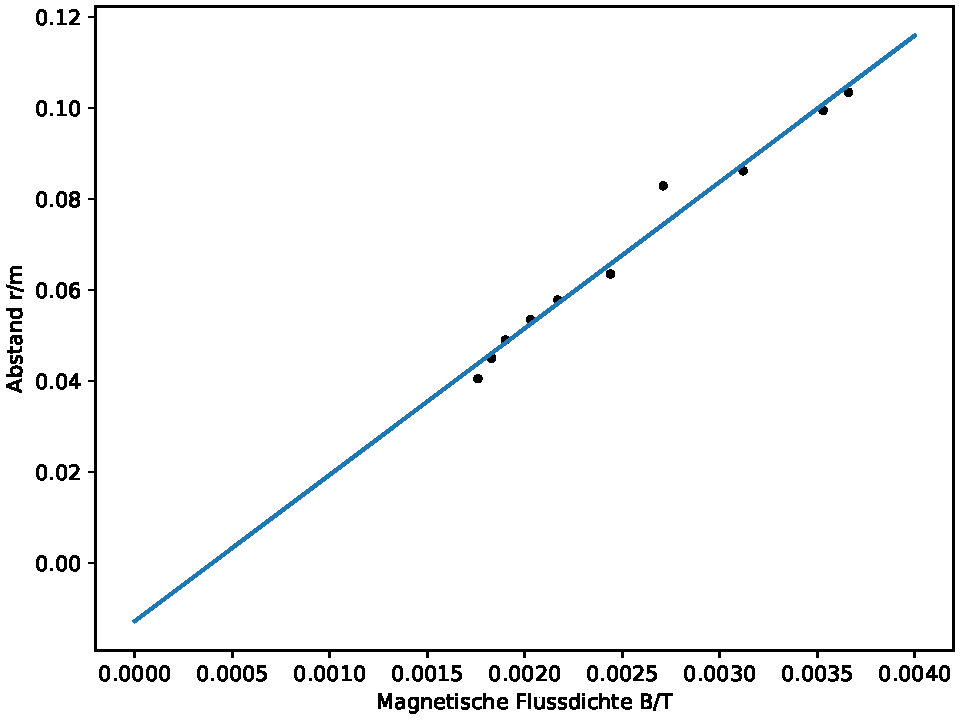
\includegraphics[width = 10cm]{plot1.pdf}
  \caption{Messwerte und lineare Regression von $r$ und $B$}
  \label{fig:plot1}
\end{figure}

Die ausgegebenen Parameter sind\\
\begin{centering}
  Steigung $a = (32.200 ± 1.639) \frac{m}{T}$\\
  Achsenabschnitt $b = (-0.013 ± 0.004)$m\\
\end{centering}

Nach \ref{eqn:grav2} wird das magnetische moment aus der Steigung als\\
\begin{centering}
  $m \cdot g \cdot a = (0.442 \pm 0.023) Am^2$\\
\end{centering}
berechnet\\
Es wurde $g = 9.81$ verwendet. %EVENTUELLLLLLLLLLL QUEEEEEEEEELLLLLLLLLLLLLEEEEEEEEEEEEEEEE
\newpage
%----------------------------------------------------------------------- ZWEITE MESSUNG

In der folgenden Tabelle \ref{tab:tabelle2} werden die Messwerte für $I$, das daraus berechnete $B$ und die Periodendauer $T_p$ aufgeführt
\begin{table}
  \centering
  \caption{Messwerte der Stromstärke, der magnetischen Flussdichte und der Periodendauer T}
  \label{tab:tabelle2}
  \sisetup{table-format=1.1, per-mode=reciprocal}
  \begin{tblr}{
      colspec = {S[table-format=3.0] S[table-format=2.1] S},
      row{1} = {guard, mode=math},
    }
    \toprule
    I \mathbin{/} \unit{\ampere} [\pm 0.1 A] & B \mathbin{/} \unit{\tesla} [\pm 0.00014 T] & T_p \mathbin{/} \unit{\second} \\
    \midrule
    0.5  & 0.00068  & 3.154 \\
    0.7  & 0.00095  & 2.557 \\
    0.9  & 0.00122  & 2.006 \\
    1    & 0.00136  & 1.948 \\
    1.3  & 0.00176  & 1.625 \\
    1.5  & 0.00203  & 1.518 \\
    1.8  & 0.00244  & 1.380 \\
    2.3  & 0.00312  & 1.174 \\
    3    & 0.00407  & 1.047 \\
    3.5  & 0.00475  & 0.892 \\
    \bottomrule
  \end{tblr}
\end{table}

Zur Bestimmung des magnetischen Momentes wird nun in Abbildung \ref{fig:plot2} eine lineare Regression der Messwerte gemacht, dabei wird $T^2$ gegen $\frac{1}{B}$ aufgetragen.
\begin{figure}
  \centering
  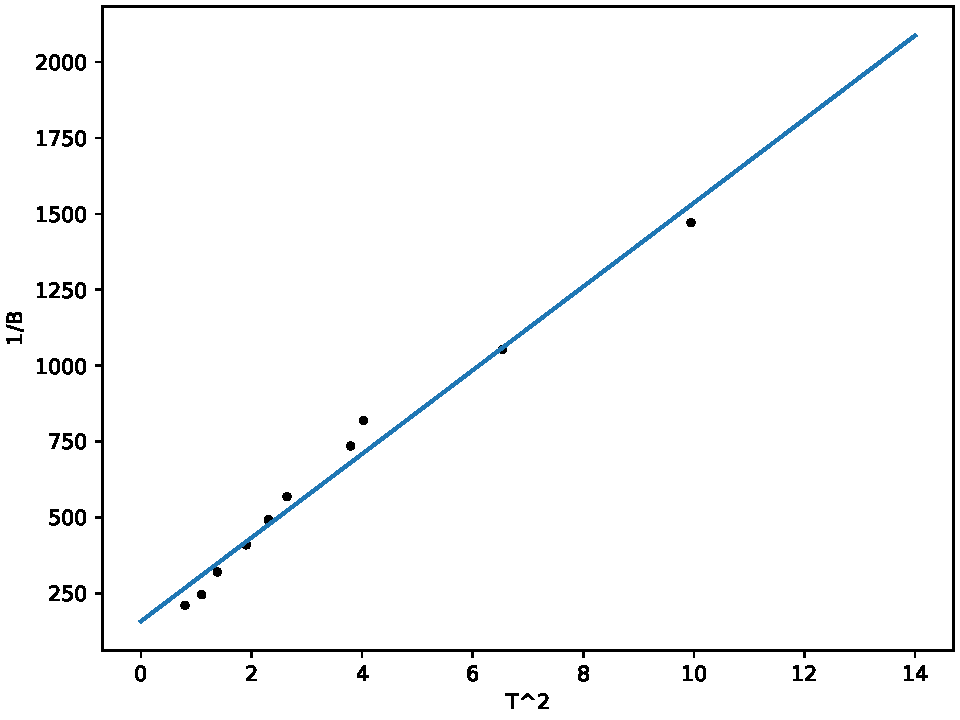
\includegraphics[width = 10cm]{plot2.pdf}
  \caption{Lineare Regression der Messwerte zur Bestimmung des magnetishen Momentes}
  \label{fig:plot2}
\end{figure}
Die von polyfit \cite{numpy} ausgegebenen Parameter sind\\

\begin{centering}
Steigung $a = (137.791 ± 6.958) s^2 \cdot T$\\
Achsenabschnitt $b = (158.221 ± 30.484) s^2$\\
\end{centering}

Das Trägheitsmoment der Billardkugel beträgt $Jk = \frac{2}{5}mr^2 = 4.704 \cdot 10^-5 kg\cdot m^2$, wie in der Vorbereitung berechnet \cite{V105}.\\

Nach \ref{eqn:schwingung1} ergibt sich das magnetsiche Moment $\mu_{\symup{o}} = (0.256 \pm 0.013) Am^2$
\newpage

%______________________________________________________-- DRITTE MESSUNG

Für die dritte Methode der bestimmung des magnetischen Momentes in der folgenden Tabelle \ref{tab:tabelle3} die Messwerte für die Periodendauern, der Mittelwert der Periodendauern,
der Stromstärke $I$ und der daraus berechneten magnetischen Flussdichte $B$ aufgeführt.
\begin{table}
  \centering
  \caption{Messwerte der Stromstärke I, magnetische Flussdichte B, und 3 Präzessionsperioden Messwerte}
  \label{tab:tabelle3}
  \sisetup{table-format=1.1, per-mode=reciprocal}
  \begin{tblr}{
      colspec = {S[table-format=3.0] S[table-format=2.1] S},
      row{1} = {guard, mode=math},
    }
    \toprule
    I \mathbin{/} \unit{\ampere} [\pm 0.1 A] & B \mathbin{/} \unit{\tesla} [\pm 0.00014 T] & T_{\symup{p}1} \mathbin{/} \unit{\second} &   T_{\symup{p}2} \mathbin{/} \unit{\second} &  T_{\symup{p}3} \mathbin{/} \unit{\second} & \symup{Mittelwert der} T_p\\
    \midrule
    1    & 0.00136  & 15.77 & 15.35 & 15.9 & 15.67   \\
    1.5  & 0.00203  & 15.5  & 17.65 & 15.6 & 16.25   \\
    2    & 0.00271  & 13.0  & 11.63 & 11.61& 12.08   \\
    2.5  & 0.00339  & 9.7   & 9.44  & 9.59 & 9.58    \\
    3    & 0.00407  & 8.54  & 7.79  & 7.42 & 7.92    \\
  
    \bottomrule
  \end{tblr}
\end{table}

In der folgenden Abbildung \ref{fig:plot3} wird mithilfe von polyfit \cite{numpy} eine lineare regression der Messwerte erstellt.
\begin{figure}
  \centering
  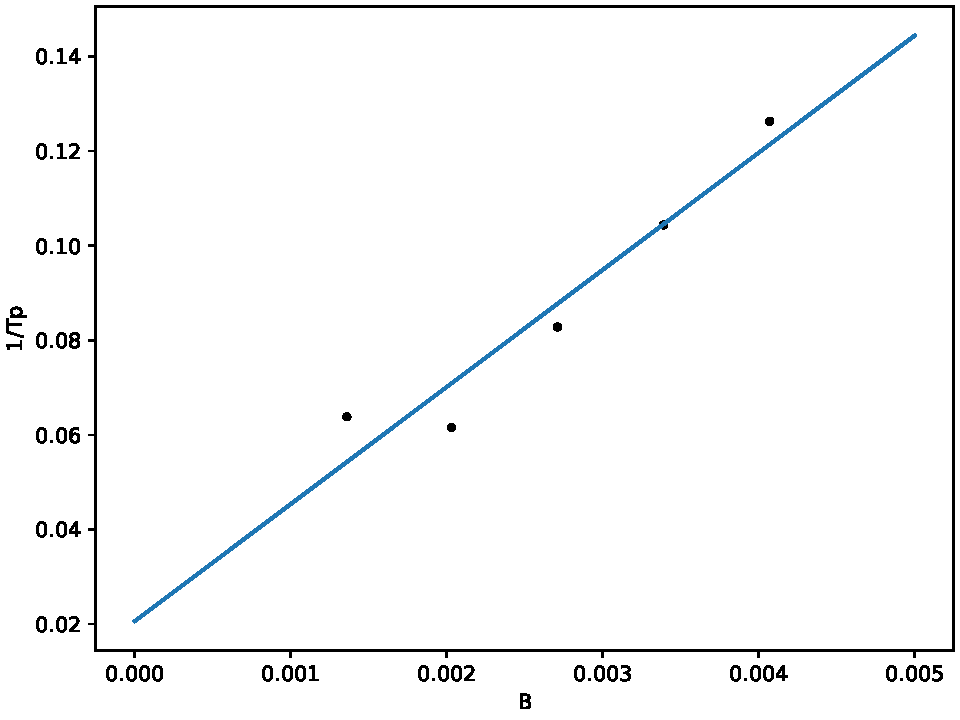
\includegraphics[width =10cm]{plot3.pdf}
  \caption{Lineare Regression zur Bestimmung des magnetischen momentes durch Präzession}
  \label{fig:plot3}
\end{figure}

Die ausgegebenen Parameter lauten\\
\begin{centering}
Steigung $a = (24.761 ± 4.049) \frac{1}{s \cdot T}$\\
Achsenabschnitt $b =(0.021 ± 0.012) \frac{1}{s}$\\
\end{centering}

Der Drehimpuls $L_{\symup{k}}$ berechnet sich mit $L_{\symup{k}} = J_{\symup{k}} \cdot \omega$ \cite{V105} zu\\

\begin{centering}

  $L_{\symup{k}} = 1.241 \cdot 10^-3 N\cdot m\cdot s$\\

\end{centering}

Damit berechnet sich das magnetische Moment nach \ref{eqn:prz1} zu\\

\begin{centering}

  $\mu_{\symup{p}} = (0.193 \pm 0.032) Am^2$\\
  
\end{centering}
 


